%%%%%%%%%%%%%%%%%%%%%%%%%%%%%%%%%%%%%%%%%%%%%%%%%%%%%%%%%%%%%%%%%%%%%%%%%%%%%%
\vspace{-2.0ex}
\section{Design and Implementation}\label{sec:des_and_impl}
%%%%%%%%%%%%%%%%%%%%%%%%%%%%%%%%%%%%%%%%%%%%%%%%%%%%%%%%%%%%%%%%%%%%%%%%%%%%%%

In this section we describe the design of MT-MPI, including
modifications to the MPICH implementation of MPI (v3.0.4) and the
Intel OpenMP runtime (version 20130412).


%%%%%%%%%%%%%%%%%%%%%%%%%%%%%%%%%%%%%%%%%%%%%%%%%%%%%%%%%%%%%%%%%%%%%%%%%%%%%%
\subsection{OpenMP Runtime}\label{sec:des-openmp}
%%%%%%%%%%%%%%%%%%%%%%%%%%%%%%%%%%%%%%%%%%%%%%%%%%%%%%%%%%%%%%%%%%%%%%%%%%%%%%

As described in Section~\ref{sec:intro}, for MPI to share OpenMP
parallelism with the application, two challenges need to be addressed.
The first is the different MPI internal algorithms that trade off
between parallelism and faster sequential execution.  The second is
the behavior of nested parallel regions in current OpenMP
implementations, including that of the Intel OpenMP runtime that is
used on Xeon Phi architectures.  Specifically, the OpenMP runtime
creates new pthreads for each nested OpenMP region, thus creating more
threads than the available cores and degrading performance.

To handle these issues, we modified the Intel OpenMP runtime to expose
the number of idle threads to the MPI implementation.  The idea is for
the OpenMP runtime system to track how many threads are being used by
the application vs. how many threads are idle (e.g., because they are
in an OpenMP barrier or outside an OpenMP parallel region).  Then, the
OpenMP runtime can provide this information through a new runtime
function.  The expectation in this model is that MPI could query for
the number of idle threads and use this information to (1) choose the
most efficient internal parallelization algorithms and (2) use only as
many threads in the nested OpenMP region as there are idle cores, by
explicitly guiding the number of threads in OpenMP (using the
\texttt{num\_threads} clause in OpenMP).

Arguably, the second challenge described above (additional pthreads
created in nested OpenMP regions) is an issue only with the current
implementation of the Intel OpenMP runtime.  An alternative OpenMP
runtime that internally uses user-level threads
(e.g.,~\cite{olivier12:openmp_qthreads}) might not face this
challenge.  However, given that most OpenMP implementations today use
pthreads internally and that Intel OpenMP is the only formally
supported OpenMP implementation on the Xeon Phi architecture, we
consider this to be a real problem that needs to be addressed.

\vspace{-1.0ex}
\subsubsection{Exposing Idle Threads}

To expose the number of idle threads in OpenMP, we need to understand
the status of threads in the following cases.

\vspace{1.0ex}
\noindent\textbf{MPI call made outside the OpenMP parallel regions}
(Figure~\ref{fig:code_hybrid_outside}).  In this case, all threads
except the main thread are idle (often equal to
\verb@OMP_NUM_THREADS@).  Thus, we expect MPI to be able
to benefit from a large number of idle threads.

\vspace{1.0ex}
\noindent\textbf{MPI call made in an OpenMP single region}
(Figure~\ref{fig:code_hybrid_single}).  OpenMP single regions provide
an implicit barrier on exit.  Thus, we can ideally expect threads to
be available ``soon'' if the number of idle threads is queried within
an OpenMP single region.  In practice, however, not all threads might
have reached the barrier yet, for example, because there is some skew
between the threads or because they are working on a user computation.
Thus, the number of idle threads available can vary anywhere between
zero and the maximum number of threads.  We modified the OpenMP
runtime to track each thread in order to return the actual number of
idle threads.  In this case, the amount of parallelism available to
MPI is unknown in the general case.  However, for OpenMP parallel
regions where the work shared between threads is mostly balanced and
threads are reasonably synchronized, the number of idle threads is
expected to be close to the maximum number of threads.

\vspace{1.0ex}
\noindent\textbf{MPI call made in an OpenMP master region or single
  region with a nowait clause} (Figure~\ref{fig:code_hybrid_master}).
This case is similar to the previous case (single region) with the
primary difference that there is no implied barrier at the end of such
a region.  Hence, there is no natural
synchronization point for the threads.  Nevertheless, depending on how
the application is written, it is possible to have an external
synchronization point (such as a user-specified OpenMP barrier) that
would cause more idle threads to be available.  Consequently, we use a
similar solution here as in the previous case, that is, to track the
number of idle threads.  In practice, however, we do not expect too
many idle threads to be available for MPI to use in this case.

\vspace{1.0ex}
\noindent\textbf{MPI call made in an OpenMP critical region}
(Figure~\ref{fig:code_hybrid_critical}).  OpenMP critical regions
force some synchronization between threads because only one thread can
enter a critical region at a time.  While this is not quite an
implicit barrier, its behavior with respect to the availability of
threads can be similar to that of an OpenMP single region.
Specifically, when the first thread enters the OpenMP critical region,
the remaining threads can be ideally expected to be idle ``soon.''  As
discussed earlier, this is not necessarily true if the other threads
are busy with the user computation or are skewed, but it can give a
reasonable model for us to consider.  When the second thread enters
the OpenMP critical region, the first thread is no longer expected to
be idle because it has already finished executing its critical region.
Similarly, when the last thread enters the critical region, none of
the remaining threads are expected to be idle because they have all
finished executing their critical regions.  As in the previous cases,
we track the number of idle threads inside the OpenMP runtime,
although we expect that the number of idle threads would be high for
the first few threads entering the critical section and low for the
last few threads.

\vspace{1.0ex}

In some of the cases described above (e.g., single region with
nowait), utilizing the idle threads can be risky because their status
can change at any time.  For example, they might have been idle
because they were in an unrelated critical section that has now
completed.  This would cause those idle threads to become active
again, degrading performance. In our implementation, we distinguish
how many threads are ``guaranteed to be idle'' and how many are
``temporarily available at the current time.''  To understand this
distinction, we need to look into when a thread can be idle.  There
are two cases when a thread can be idle: (1) if it is waiting in a
barrier waiting for other threads in the team to arrive or (2) if it
is outside a critical section waiting to enter it.

A thread that is in a barrier is guaranteed to be idle till all other
threads in that team reach the barrier.  Thus, when a thread in that
team queries for the number of guaranteed idle threads, all the
threads that are waiting in the barrier will contribute to the
returned value.  Waiting to enter a critical section is a bit more
tricky in that a thread is guaranteed to wait only till the thread
that is already in the critical section does not exit the critical
section.  Thus, if the thread that is already in the critical section
queries for the number of guaranteed idle threads, the threads waiting
to enter the critical section will contribute to the returned value.
For all other threads, the threads waiting to enter the critical
section will not contribute to the guaranteed idle threads but will
contribute to the temporarily available threads.

Thus, the following semantics hold true for the number of guaranteed
idle threads:

\begin{enumerate}
\setlength{\parskip}{-0.2ex}
\vspace{-1.0ex}

\item It is thread-specific.  At a given point of time, depending on
  which thread is querying for the information, the returned value
  might be different (it can increase or decrease).

\item It is OpenMP-region specific.  If the querying thread enters a
  new OpenMP region (e.g., critical or single) or exits it, the
  returned value might be different (it can increase or decrease).

\item It is time-specific.  At two different points of time the
  returned value might be different (e.g., if more threads reached a
  barrier).  However, if the same thread queries for the value and it
  is in the same OpenMP region, the value can only increase, not
  decrease.

\vspace{-1.0ex}
\end{enumerate}

We modified the OpenMP runtime to keep track of which type of OpenMP
region each thread is in, in order to return both the guaranteed
number of idle threads and the number of temporarily idle threads.  We
note that our implementation treats a thread as idle only when it is
not engaged in any OpenMP activity, including OpenMP parallel loops
and OpenMP tasks.  We also note that in our implementation the
performance overhead associated with tracking whether a thread is
actively being used by the OpenMP runtime is too small to be observed
and hence is not demonstrated in this paper.


\subsubsection{Thread Scheduling for Nested Parallelism}

For well-balanced OpenMP parallel loops with little to no skew, thread
synchronizations such as barriers are often short-lived because
threads tend to arrive at the barrier at approximately the same time.
Thus, when a thread arrives at a barrier, if it is put to sleep while
waiting for the other threads to arrive, only to be woken up in a
short amount of time, performance is degraded because of the cost of
waking up threads from a sleep state.  To work around this situation,
the Intel OpenMP runtime does not put threads to sleep immediately
when they reach a barrier.  Instead, they spin waiting for other
threads to arrive, for a configurable amount of time:
\verb@KMP_BLOCKTIME@.  A large value for this variable would mean that
threads do not become truly idle for a long time.  While this
situation is not a concern for regular OpenMP parallel loops, it can
degrade performance for nested OpenMP parallel loops since the Intel
OpenMP runtime creates more threads than the number of cores in such
cases.  Having the primary threads spin for \verb@KMP_BLOCKTIME@ would
cause more threads to be active than the number of available cores for
that much time.

When MPI calls are outside the application OpenMP parallel region
(such as in Figure~\ref{fig:code_hybrid_single}), this is not a
concern since MPI would use the same threads as the application in its
parallel region.  When MPI calls are inside the application parallel
region, however, this would require MPI to use a nested OpenMP
parallel region.  And since the threads that arrived at the barrier
would not yield the available cores immediately, this would either
require MPI to utilize lesser parallelism by only using the idle cores
or cause thread thrashing on the available cores for
\verb@KMP_BLOCKTIME@ amount of time.  Neither solution is
ideal.

In MT-MPI, to be able to employ these resources as soon as possible,
we implemented and exposed a new function in the OpenMP runtime:
\verb@set_fast_yield@.  This function plays two roles.  First, it
forces the threads in the current team to skip the active wait during
the barrier operation and immediately yield the core.  Second, it
continuously yields the core using \verb@sched_yield@ calls instead of
simply sleeping.  We used this approach primarily because of the
overhead associated with sleep vs. that of yield.  We found that
yielding allows us to manage the cores with a much lower overhead
(about 30 $\mu$s even with 240 threads) compared with sleeping (more
than 100 $\mu$s even at 16 threads).

We note that (1) our thread scheduling optimization impacts only
those threads that are guaranteed to be idle (e.g., threads waiting in
an OpenMP barrier); (2) the fast yield setting is performed internally
inside the MPI call and reset once the internal parallelism in MPI is
complete, so future OpenMP barriers are not affected by it; and (3)
the proposed thread scheduling optimization affects only that case
when MPI uses nested OpenMP parallelism (e.g., when an MPI function
is called in an OpenMP single region) and does not affect the case
when the MPI function is called outside the OpenMP parallel region.


%%%%%%%%%%%%%%%%%%%%%%%%%%%%%%%%%%%%%%%%%%%%%%%%%%%%%%%%%%%%%%%%%%%%%%%%%%%%%%
\subsection{MPI Internal Parallelism}\label{sec:des-mpi}
%%%%%%%%%%%%%%%%%%%%%%%%%%%%%%%%%%%%%%%%%%%%%%%%%%%%%%%%%%%%%%%%%%%%%%%%%%%%%%

Using the information about the idle threads exposed by our extended
OpenMP runtime, the MPI implementation can schedule its internal
parallelism efficiently to obtain performance improvements. In this
section, we demonstrate the benefit of such internal parallelism for
various aspects of the MPI processing, including derived datatype
communication, shared-memory communication, and network I/O
operations.  In our MPI implementation, we utilize only those idle
thre\-ads that are guaranteed to be available.  Although here we do
not utilize temporarily available threads, one could envision cases
(e.g., short MPI operations) where they could be.  In our
implementation, when all threads are idle (e.g., when the MPI call is
outside the OpenMP parallel region), we do not specify the number of
threads to be utilized by OpenMP; instead, we let it manage such
parallelism internally.  If fewer than the maximum number of threads
is idle, however, we direct the amount of thread parallelism to use
through the \texttt{num\_threads} OpenMP clause.


%%%%%%%%%%%%%%%%%%%%%%%%%%%%%%%%%%%%%%%%%%%%%%%%%%%%%%%%%%%%%%%%%%%%%%%%%%%%%%
\subsubsection{Derived Datatype Processing}\label{sec:imp-ddt}
%%%%%%%%%%%%%%%%%%%%%%%%%%%%%%%%%%%%%%%%%%%%%%%%%%%%%%%%%%%%%%%%%%%%%%%%%%%%%%

MPI allows applications to describe noncontiguous regions of memory
using user-derived datatypes such as \textit{vector},
\textit{indexed}, and \textit{struct}.  These derived datatypes can be
used to describe arbitrarily complex data layouts to be processed by
MPI for packing/unpacking data to/from a contiguous buffer (using
\texttt{MPI\_PACK} and \texttt{MPI\_UNPACK}) or to send/receive data.
When communicating using derived datatypes, MPI implementations
typically internally pack data into contiguous buffers, communicate
these contiguous buffers, and internally unpack them into the
recipient buffer.  Halo exchanges~\cite{halo} are a well-known example
of communications that are well suited to employ derived datatypes.

The pack and unpack processing stages consist of a set of local memory
copies.  A typical implementation traverses the derived datatype tree
and copies each noncontiguous chunk of data separately.  Some
implementations of MPI optimize such processing by representing the
entire datatype as a stack structure so that it can be iteratively
traversed rather than using a recursive traversal~\cite{mpi-dataloop}.
Given that each noncontiguous data chunk is copied to a different
location and there are no dependencies among the different data
elements, such copies are a good candidate for OpenMP parallelization.
Moreover, thanks to the relatively large private caches per core on
the Xeon Phi architecture, concurrent accesses to separate memory
regions by the different threads are expected to be highly efficient.
Therefore, we modified the MPI implementation to parallelize the
datatype data copy using OpenMP.  We note that only the lowest level
of a nested datatype (e.g., a vector of vectors) is parallelized in
MT-MPI.

\newsavebox\codeSequentialPackBox
\begin{lrbox}{\codeSequentialPackBox}
\begin{lstlisting}[linewidth=0.44\columnwidth]
for (i=0; i<count; i++){
  *dest++ = *src;
  src += stride;
}
\end{lstlisting}
\end{lrbox}

\newsavebox\codeParallelPackBox
\begin{lrbox}{\codeParallelPackBox}
\begin{lstlisting}[linewidth=0.51\columnwidth]
#pragma omp parallel for
for (i=0; i<count; i++){
  dest[i] = src[i * stride];
}
\end{lstlisting}
\end{lrbox}

\begin{figure}[t]
\centering
\subfigure[Sequential implementation.] {
  \usebox\codeSequentialPackBox
  \label{fig:code-seq-pack}
}
\hspace{0.2ex}
\subfigure[Parallel implementation.] {
  \usebox\codeParallelPackBox
  \label{fig:code-para-pack}
}
\vspace{-1.5ex}
\caption{Sequential and parallel data packing.}
\vspace{-3.5ex}
\end{figure}

One issue that we found using MT-MPI was an unintended consequence of
the compiler vectorization.  The original data\-type copy code that is
used in MPICH is shown in Figure~\ref{fig:code-seq-pack}.  While this
code works correctly for sequential data copy, it cannot be easily
parallelized by using OpenMP because the compiler cannot understand
the constant stride of accesses used through all iterations.  We
therefore modified the code as shown in
Figure~\ref{fig:code-para-pack}.  While this new implementation makes
it easier for the compiler to understand the computation and thus
parallelize it, the implementation also makes it easier for the
compiler to vectorize the code.  This situation in itself is not a
concern.  However, the Intel compiler is inefficient in vectorizing
strided loops with large stride values when the amount of data copied
in each loop is small.  Specifically, the compiler does incorrect
prefetching in this case, causing additional cache misses and thus
losing performance.  Consequently, our modification to the code is not
always beneficial and can perform worse than the sequential
implementation when very few threads are available.  To work around
this issue, we could either disable vectorization in the parallel
implementation or explicitly choose only the parallel approach when a
sufficiently large number of threads are available.  We chose the
latter approach because vectorization is still beneficial in some
cases (e.g., when the stride is small or the copy size is large).

We note that the incorrect cache prefetching and additional cache
misses that it causes have been experimentally verified, but the
results are not shown in this paper because of space restrictions.
The issue has also been reported to Intel and has been confirmed by
their compiler team.  They are expected to fix it in a future release
of the compiler.

%%%%%%%%%%%%%%%%%%%%%%%%%%%%%%%%%%%%%%%%%%%%%%%%%%%%%%%%%%%%%%%%%%%%%%%%%%%%%%
\subsubsection{Shared-Memory Communication}\label{sec:imp-lmt}
%%%%%%%%%%%%%%%%%%%%%%%%%%%%%%%%%%%%%%%%%%%%%%%%%%%%%%%%%%%%%%%%%%%%%%%%%%%%%%

When multiple MPI processes reside on the same node, since each
process has a different virtual address space, most MPI
implementations, including MPICH, use a pipelined double-copy strategy
through shared memory for intranode communication~\cite{mpich-lmt}.
As shown in Figure~\ref{fig:shd_pipeline}, a shared-memo\-ry ring buffer
is allocated between the sender and receiver processes and divided
into multiple cells; the sender process then copies part of data into
an empty cell while the receiver process copies a full cell out.

\begin{figure}[h]
  \vspace{-2.0ex}
  \subfigure[Sequential pipelining.] {
    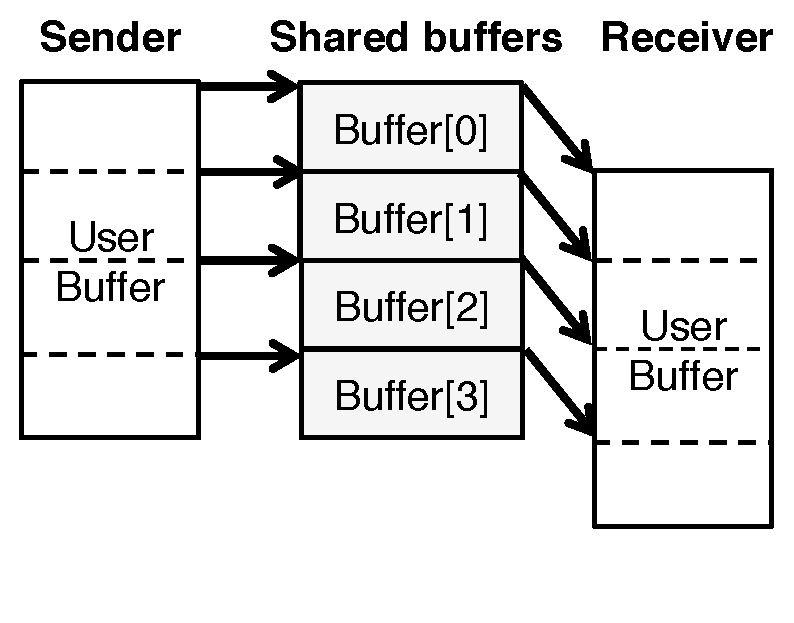
\includegraphics[width=0.43\columnwidth]{figures/mtmpi/imp-shared-pipeline.pdf}
    \label{fig:shd_pipeline}
  }
  \hfill
  \subfigure[Parallel pipelining.] {
    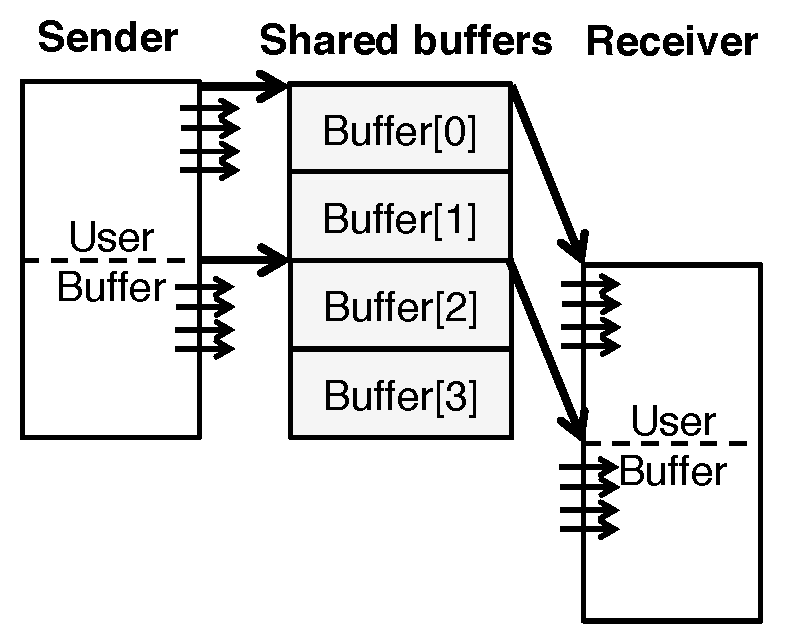
\includegraphics[width=0.43\columnwidth]{figures/mtmpi/imp-shared-parallel-pipeline.pdf}
    \label{fig:shd_parallel_pipeline}
  }
  \vspace{-2.0ex}
  \caption{Data movement of parallelization and pipelining.}
  \vspace{-2.0ex}
  \label{fig:shd_parallel_datamove}
\end{figure}

In MT-MPI, we parallelize this copy on both the sender and the
receiver side using the available idle threads.  We implemented this
optimization by extending the pipelined double-copy strategy used
within MPICH.  As shown in Figure~\ref{fig:shd_parallel_pipeline}, in
our approach we reserve multiple contiguous available cells and
concurrently copy data from the user buffer to these cells on the
sender side and from the cells to the user buffer on the receiver
side.  For messages larger than what can be held in the reserved
cells, additional pipelining is used, similar to the sequential case.
Compared with the sequential pipelining algorithm, however, the
parallel algorithm can degrade performance in the following cases.

\vspace{1.0ex}
\noindent\textbf{Small messages.}  When the message size is small,
there is not enough work in MPI to be parallelized.  In such cases,
the thread management and synchronization within OpenMP are more
expensive than the sequential copy mechanism already used in MPICH.
Thus, in this case we do not expect any performance benefit from
parallelization.

\vspace{1.0ex}
\noindent\textbf{Large messages but few idle threads.}  In our
parallel implementation, we reserve as many shared-memory cells as
possible and parallelize the copy using all of the available idle
threads.  Thus the receiver process now has to wait until data is
filled into all of the reserved cells before it can start its data
copy out of shared memory.  This approach, in essence, increases the
pipeline unit to a much larger size.  Thus, while parallelism can
improve the performance of each memory copy operation, it can also
hurt the data copy pipeline.  We note that we cannot simply reduce the
size of each shared-memory cell or the maximum number of cells
reserved to work around this issue because that would reduce the
amount of work done by each thread, thus causing the thread management
overhead to dominate.  This trend is illustrated in
Figure~\ref{fig:shd_timing}.  Specifically, compared with sequential
pipelining (Figure~\ref{fig:shd_pipeline_timing}), when the number of
threads available to MPI is small, the parallel copy does not improve
performance much but delays the receiver process from getting started
with its copy (Figure~\ref{fig:shd_poor_para_timing}).  On the other
hand, when a large number of threads are available to MPI, the parallel
copy is significantly faster, thus balancing the loss of performance
due to the reduced pipelining (Figure~\ref{fig:shd_para_timing}).

\begin{figure}
  \subfigure[Sequential pipelining.]{
  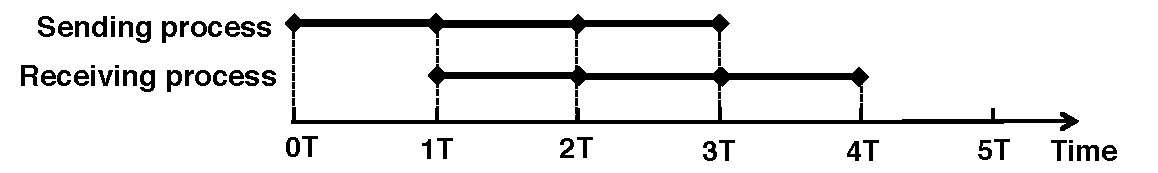
\includegraphics[width=0.95\columnwidth]{figures/mtmpi/imp-shared-pipeline-timing.pdf}
  \label{fig:shd_pipeline_timing}
  }
  \subfigure[Poor parallelism.]{
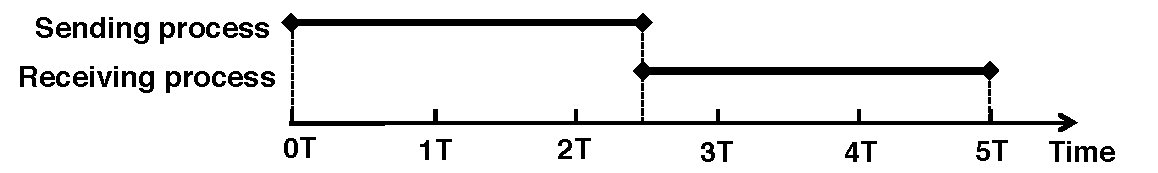
\includegraphics[width=0.95\columnwidth]{figures/mtmpi/imp-shared-poor-para-timing.pdf}
  \label{fig:shd_poor_para_timing}
  }
  \subfigure[Strong parallelism.]{
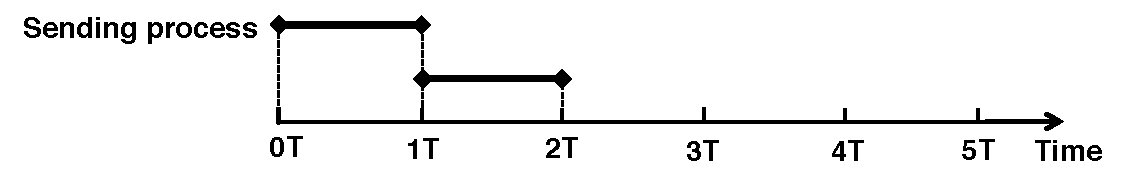
\includegraphics[width=0.95\columnwidth]{figures/mtmpi/imp-shared-para-timing.pdf}
  \label{fig:shd_para_timing}
  }
  \vspace{-2.0ex}
  \caption{Sequential pipelining vs. parallel data copy.}
  \vspace{-3.0ex}
  \label{fig:shd_timing}
\end{figure}

\vspace{1.0ex}
\noindent\textbf{Few shared-memory cells.}  The amount of data to be
copied is decided not just on the number of available threads but also
on the number of available shared-memory cells.  Specifically, during
the communication process, some cells might be in use for transferring
previous messages (or previous parts of the same message).  In such
cases, there is not enough work to be parallelized, and hence the
thread management would add too much overhead to justify the
performance improvement through parallelization.
\vspace{1.0ex}

In summary, parallelism would improve performance only when (1) the
message size is not too small ($\ge$ 64~Kbytes), (2) the number of
threads is not too few ($\ge$ 8), and (3) the total size of free cells
is not too small ($\ge$ 64~Kbytes). In our implementation, we utilize
the parallel shared-memory communication algorithm only when all three
conditions are met; otherwise we fall back to the original sequential
algorithm.  We note that the above-mentioned thresholds are
empirically evaluated on our test platform and must be tuned for
different platforms.


%%%%%%%%%%%%%%%%%%%%%%%%%%%%%%%%%%%%%%%%%%%%%%%%%%%%%%%%%%%%%%%%%%%%%%%%%%%%%%
\subsubsection{Optimizations for the InfiniBand Network}\label{sec:imp-netmod}
%%%%%%%%%%%%%%%%%%%%%%%%%%%%%%%%%%%%%%%%%%%%%%%%%%%%%%%%%%%%%%%%%%%%%%%%%%%%%%

Several MPI implementations are optimized for a variety of networks
through a layered software architecture where one of the layers
provides network-specific functionality.  In MPICH, this layer is
called the \texttt{netmod layer}.  Multiple netmod implementations
exist for MPICH over InfiniBand (IB), with more-or-less similar
functionality and performance.  In this paper we utilize the
implementation described in~\cite{mpich-ibnetmod}.

An MPI implementation utilizing IB needs to create and manage a number
of objects, including contexts, protection domains (PDs), queue pairs
(QPs), and completion queues (CQs).  A process can create one or more
IB contexts, each of which maintains a collection of state information
associated with the communication.  Each context can contain one or
more PDs, each of which defines the protection semantics of memory and
other objects used by the program, for example to allow different
connections access to different sets of memory regions.  Within a PD,
the program can create one or more QPs, each of which consists of a
send queue and a receive queue.  A QP is used to communicate between a
pair of processes.  A PD can also have one or more CQs, each of which
is used to check for the completion of communication operations on one
or more QPs.  IB also provides shared queues for better memory
management, but for simplicity we do not describe them here.

The IB software stack~\cite{ofed} is thread-safe.  When multiple
threads access the same QP or CQ, it internally uses mutexes to
maintain state consistency.  Such state consistency is expensive,
however, and can degrade performance.  Therefore, in our approach we
try to avoid such usage and instead have different threads manage
different QPs in order to maximize performance.  Even with this
approach some shared data structures still need to be protected.  To
understand how much performance improvement MPI can gain by
parallelizing the posting of network operations, we studied how much
potential parallelism there is in the IB stack that can theoretically
be exploited.  We modified the {\tt ib\_write\_bw} benchmark from the
OpenFabrics Enterprise Distribution (OFED) package~\cite{ofed} to
measure the multithreaded point-to-point IB RDMA write bandwidth
between two Intel Xeon Phi coprocessors on different nodes.  We define
three parallelism levels:

\vspace{1.0ex}
\noindent\textbf{IB contexts.}  Each process has 64 IB contexts, and
each context has one QP and one CQ.  Each thread handles operations on
a different context, CQ and QP.

\vspace{1.0ex}
\noindent\textbf{QPs and CQs.}  Each process has a single IB context
with 64 QPs and 64 CQs.  Each CQ is dedicated to a different QP.  Each
thread handles operations on different QPs and CQs, but they all share
the same context.

\vspace{1.0ex}
\noindent\textbf{QPs only.}  Each process has a single IB context with
64 QPs and one shared CQ.  Each thread handles operations on different
QPs, but they all share the same context and CQ.

\begin{figure}[h]
\vspace{-2.0ex}
\centering
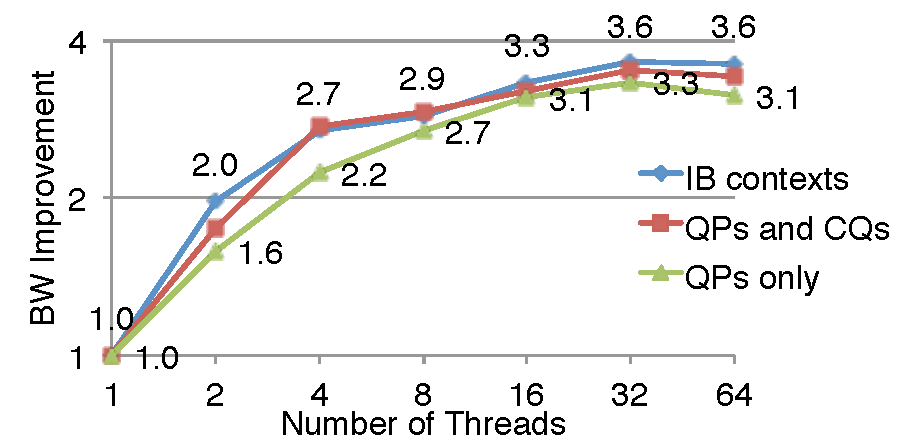
\includegraphics[width=0.8\columnwidth]{figures/mtmpi/imp-stp-ib-write-bw.pdf}
\vspace{-2.0ex}
\caption{Small (64-byte) IB RDMA write bandwidth.}
\label{fig:imp-ib-write-bw}
\vspace{-2.0ex}
\end{figure}

Figure~\ref{fig:imp-ib-write-bw} compares the communication bandwidth
of small messages (64 bytes) for the cited parallelism levels.  We
make two primary observations from the figure.  The first is that the
performance improvement with increasing threads is higher when the
number of shared resources is less.  For example, when each thread has
a separate context (\texttt{IB contexts}), with increasing threads,
the parallel performance is 3.6-fold higher than the sequential
performance.  But when the context and the CQ are shared by all
threads (\texttt{QPs only}), the parallel performance is only 3.1-fold
higher than the sequential performance.  This result is expected
because more sharing typically means more critical sections and hence
more serialization.  The second observation is that the maximum
parallelism that the IB-stack can provide is 3.6-fold when all
resources are dedicated per thread and 3.1-fold when the context and
CQ are shared between all the threads.  Most MPI implementations are
increasingly moving toward more shared resources (i.e., closer to
\texttt{QPs only}) in order to manage the per-process resource usage.
Thus, in current MPI implementations, 3.1-fold improvement is the
maximum benefit that we can expect even in the ideal case.

In MT-MPI, each QP is managed by a single thread; multiple QPs might
be managed by a single thread, but a single QP is never managed by
multiple threads.  This strategy minimizes the mutexes that the IB
stack needs to do.  We also ensure that the number of threads used for
parallelism is never more than the number of QPs, in order to minimize
thread synchronization overheads.

We note that in the MPICH IB netmod, small-message communication
employs temporary buffers that are preregistered with the network.
Since the network can communicate only to/from preregistered buffers,
user data needs to be copied into these buffers on the sender side and
out of these buffers on the receiver side.  Each connection uses a
separate QP and preregistered buffers, so the data copies on the send
and receive side are also part of the parallelism and are executed
concurrently by different threads.

Despite the potential for parallelism on many-core architectures,
several factors limit the practical parallelism
achievable in the MPI implementation.  For example, in order to
achieve the best parallelism, the MPI implementation can benefit from
a large number of operations to be issued to the network, which can be
evenly shared between the available threads.  However, such ideal
conditions are hampered by several practical restrictions in current
IB network stacks and applications.  For example, the number of
operations that can be issued to a QP or to the shared CQ is limited.
While the QP or CQ can be configured to allow for a large number of
operations, such configuration causes (sometimes large) performance
degradation due to the internal bookkeeping associated with these data
structures within the IB stack.  Consequently, the MPICH IB netmod
configures this limit to 1,024 for QPs and 32,768 for CQs, thus
forcing the maximum number of network operations each thread can post
to 1,024 and the maximum number of network operations posted across
all threads to 32,768, before thread synchronization is needed.  A
similar parallelism-limiting factor is the number of preregistered
buffers available at the sender and receiver side.

Still another parallelism constraint comes from the application
characteristics.  Specifically, since in MT-MPI we exploit parallelism
at the granularity of a QP, for ideal parallelism we need the same
amount of work per QP---a process should have close to uniform
communication with its peer processes.  In practice, however, this
assumption does not hold; indeed, the amount of communication can vary
dramatically between different processes, thus limiting the available
parallelism.
